\section{Laboratory Lecture 8: Integrated Circuit Technologies}

\subsection{Introduction}

The main objective of this practice is to get a grasp of the most important characteristics of logic families and their usage in real-life circuits.\medskip

As we have discussed in previous practices, logic gates are a staple in the field of digital electronics. Something that we have not discussed until know is the concept of \textbf{\textit{logic families}}. \medskip

During the production of digital integrated circuits, different circuit configurations and production technologies are used. Each of these approaches can be refered to as a specific \textbf{logic family}. The idea behind having different approaches, or different logic families, is that each IC of same family will have identical electrical characteristics, and because of that, will be compatible with each other. These characteristics, which are bound to be identical, are, for instace, supply voltage range, speed of response, power dissipation, input and output logic levels, current sinking and sourcing capability, noise margin, fan-out, to name a few.\medskip

Nowadays, there are 2 important logic families that comprise most of the ICs that one may find, namely \textbf{\textit{Bipolar families}} and \textbf{\textit{MOS (Metal oxide semiconductor) families}}. The first family is formed by technologies such as diode logic (DL), emitted coupled logic (ECL), resistor transistor logic (RTL), diode transistor logic (DTL), transistor transistor logic (TTL), whereas the latter is composed of PMOS, NMOS, CMOS. There is also a special type of logic family that combines both bipolar and CMOS, called Bi-CMOS. \medskip

Out of the above mentioned families DL, RTL and DTL are not used these days, as they have become obsolete. TTL, CMOS, ECL, NMOS and Bi-CMOS, on the other hand, continue to be used in electronic devices nowadays.\medskip

In general, CMOS devices have greater noise immunity and draw less power, due to the way in which the internal switching is performed, i.e. by applying a specific voltage to the gate of the FET, as opposed to TTL devices, which require polarizing currents to operate. Besides, due to the insignificant power draw, the CMOS family dissipates less energy as heat. \medskip

The term \textbf{\textit{noise inmunity}} refers to the circuit's ability to tolerate noise, i.e.unwanted voltages which are normally induced in logic circuits by electric/magnetic fields, without changes. As we have said, the noise inmunity of CMOS devices is greater than the one of TTL devices. We can see this in the following image. \medskip


\begin{figure}[H]
    \centering
    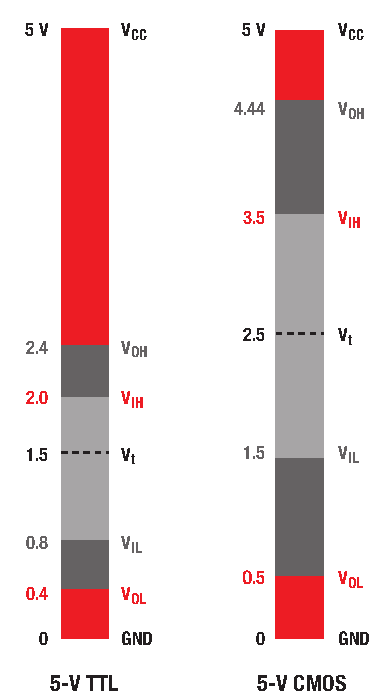
\includegraphics[scale = 0.8]{Graphics/Practice 8/TTL_VS_CMOS.pdf}
    \caption{TTL vs CMOS noise margins~\autocite{LOGIC_GUIDE}}
    \label{fig:TTL_VS_CMOS}
\end{figure}

In this image we can see the different voltage levels that define each family. A brief definition of each one can be found below:

\begin{itemize}
    \item $\mathbf{V_{OH (MIN)} - \text{High-Level Input Voltage}}$: The minimum voltage level require for a logic 1 at the \textit{input}. Any voltage below this level will not be accepted as a HIGH by the logical circuit. 

    \item $\mathbf{V_{IL (MAX)} - \text{Low-Level Input Voltage}}$: The maximum voltage level require for a logic 0 at the \textit{input}. Any voltage above this level will not be accepted as a LOW by the logical circuit. 

    \item $\mathbf{V_{OH (MIN)} - \text{High-Level Output Voltage}}$: The minimum \textit{output} voltage for a logic 1 under defined load conditions.

    \item $\mathbf{V_{OL (MAX)} - \text{Low-Level Output Voltage}}$: The maximum \textit{output} voltage for a logic 0 under defined load conditions.
\end{itemize}

For proper operation, logic circuit input voltage levels must be kept out of the indeterminate range, i.e. lower than $\mathbf{V_{IL (MAX)}}$ or higher than $\mathbf{V_{IH (MIN)}}$.\medskip

To calculate the noise inmunity, we have to calculate both the High-state noise margin and the Low-state one. The difference between the tolerable output and input ranges is called the noise margin of the gate. 

\begin{align*}
    V_{NH} &= V_{OH (MIN)} - V_{OH (MIN)} \\
    V_{NL} &= V_{IL (MAX)} - V_{OL (MAX)}
\end{align*}\medskip


Before diving into the practice itself, we will briefly go over the main components that will be used in this practice.

\subsubsection{Inverter Logic Gate: 74HCT04}

74HCT04 is nothing more than an array of 6 CMOS inverter logic gates with standard push-pull outputs. \medskip

From the datasheet~\autocite{74HCT04}, we can obtain the values of the parameters that we described ealier. 

\begin{table}[ht]
    \centering
        \begin{tabular}[t]{lcccc}
            \toprule
            & \textbf{Symbol} & \textbf{Parameter} & \textbf{Min} & \textbf{Max} \\
            \midrule
            & $V_{IH}$ & High-Level Input Voltage  & 2.0         &             \\
            & $V_{IL}$ & Low-Level Input Voltage   & \textendash & 0.8         \\
            & $V_{OH}$ & High-Level Output Voltage & 4.4         & \textendash \\
            & $V_{OL}$ & Low-Level Output Voltage  & 3.8         & \textendash \\
            \bottomrule
        \end{tabular}
        \caption{74HCT04 CMOS Voltage Levels}
        \label{table:74HCT04_VOLT_LEVELS}
\end{table}

These values will be used later on in the practice.

\subsubsection{BJT: BD315}

Transistors, in general, are 3 terminal active devices made from different semiconductor materials such as silicon or germanium that can act as either an insulator, or a conductor, depending on the electrical signal that is supplied to them. The transistor’s ability to change between these two states enables it to have two basic functions: \textbf{\textit{switching}} (digital electronics) or \textbf{\textit{amplification}} (analogue electronics)\medskip

There are 2 major types of transistors, namely \textbf{BJTs} and \textbf{FETs}. BJT stands for \textbf{Bipolar Junction Transistor} whereas FET stands for \textbf{Field-Effect Transistor}. The first type of transistors are controlled by sourcing or sinking current to their base terminal (NPN or PNP, respectively), unlike the latter, which are controlled by applying a voltage, to their gate terminal (NMOS or PMOS). \medskip

Transistors are one of the most important components in electronics, as they are used in almost every active component. Logic gates, for instance, use transistors to perform the internal switching operations. As saw in the last section, TTL devices use BJTs, and CMOS use FETs.\medskip

The \textbf{BD135} can be described as an NPN BJT. As we have said, BJTs are controlled by current. In the case of NPNs, a small current has to be supplied to their base terminal for them to work. PNPs, on the other hand need to have some current sinked out of their base terminal for them to work properly.\medskip

\clearpage

Depending on the amount of current that one sinks/sources, to/from their base terminal, they will operate in different regions, namely:

\begin{itemize}
    \item \textbf{Active Region:} The transistor behaves as an amplifier. 
    \item \textbf{Saturation:} The transistor behaves as a switch.
    \item \textbf{Cut-off:} The transistor is OFF $\rightarrow$ No current flow.
\end{itemize}

This 3 operation modes can be seen in the following image:

\begin{figure}[H]
    \centering
    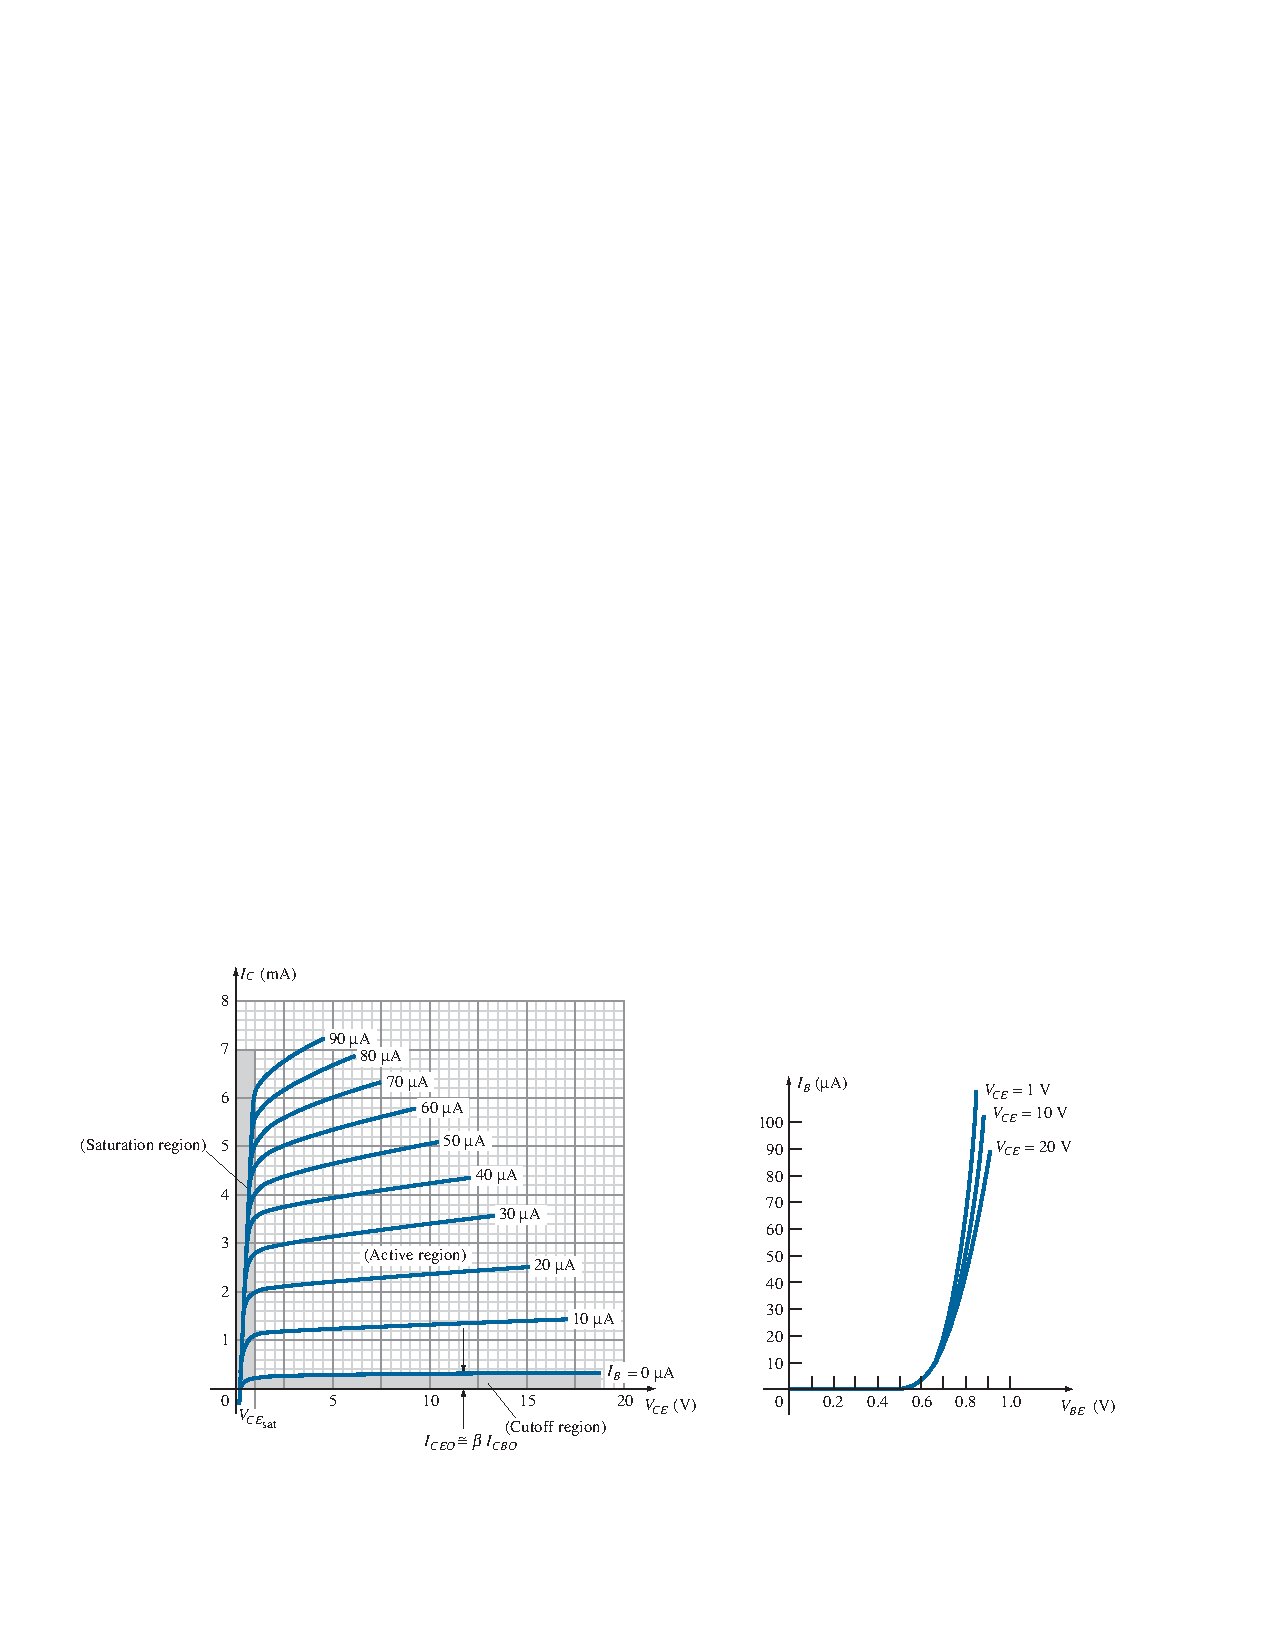
\includegraphics[width = \textwidth]{Graphics/Practice 8/BJT/IC_VCE.pdf}
    \caption{BJT (NPN) operation modes~\autocite{BOYLESTAD}}
    \label{fig:BJT_MODES}
\end{figure}


As it can be seen in the graph, the active region represents a zone in which the colector current is proportional to the base current. This relationship can be expressed by the following equation:

\begin{equation*}
    I_C = \beta \cdot I_B
\end{equation*}

\noindent Where $\beta$ is the gain, a value that can be considered constant for each transistor and $I_C$ and $I_B$ are the collector and base currents respectively. \medskip

An example circuit can be seen below:

\begin{figure}[H]
    \centering
    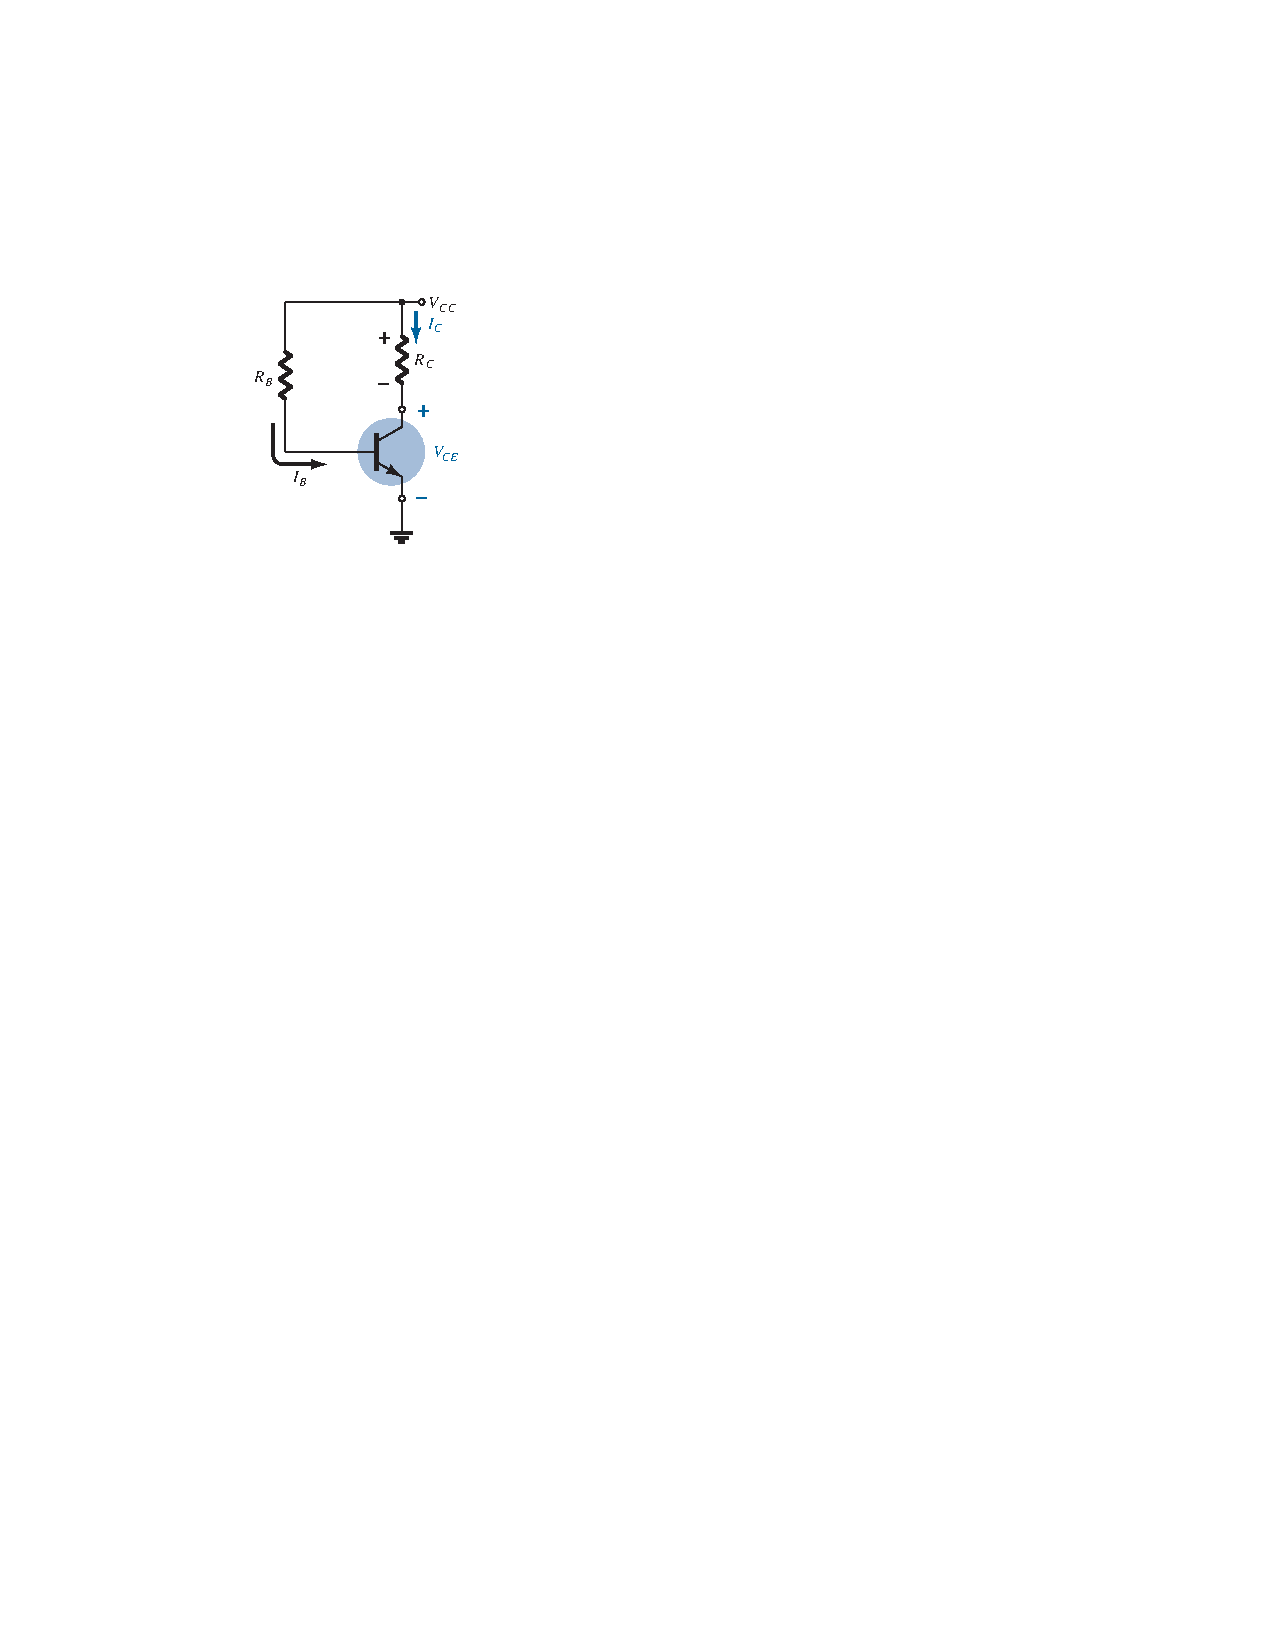
\includegraphics[scale = 1]{Graphics/Practice 8/BJT/NPN_CIRCUIT.pdf}
    \caption{NPN example circuit~\autocite{BOYLESTAD}}
    \label{fig:NPN_EXAMPLE}
\end{figure}

The $V_{CE}$, or the Collector-to-Emitter voltage, is also plotted in the image. As the current that passes through the load, $I_C$, increases, the $V_{CE}$ decreases, that is, the more power that the load dissipates, the less power that the BJT has to dissipate. There is a point in which the equation described above does not hold anymore. This critical point is reached when the $I_C$ is maximum, and so the $V_{CE}$ is minimum. If more base current were to be sourced to the base of the NPN, the $I_C$ would NOT increase linearly.\medskip

Once this point is reached, the NPN is in Saturation, i.e., it behaves like a switch. In this operation mode, the $V_{CE} \approx 0.1-0.2 \; V$, and the $V_{BE} \approx 0.8 \; V$.

\subsection{Exercise 1: Light Control}

\textit{\textbf{Exercise 1:}} \textit{It is wanted to design a light control by using a LDR (Light Dependent Resistor). The system has to have an input interface circuit in order to adapt the LDR signal. When the LDR works in an absolutely darkness or in a complete brightness, the interface circuit has to work with HCT compatible logic levels.}

\begin{figure}[H]
    \centering
    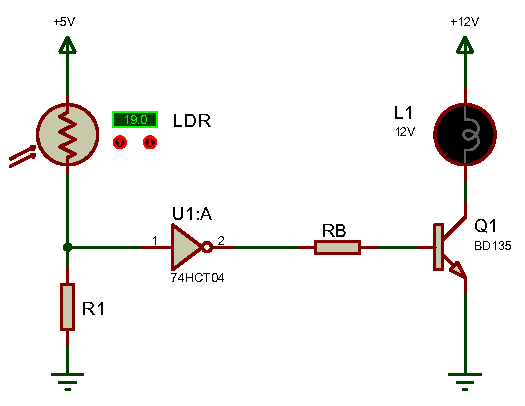
\includegraphics[scale = 0.9]{Graphics/Practice 8/EXERCISE_1/EX_1.PDF}
    \caption{Exercise 1 Assembly}
    \label{fig:EX_1}
\end{figure} \medskip

The ohmic values of the LDR are given:

\begin{itemize}
    \item $R_{LDR} \left( \text{brightness} \right) = 3.5 \; k\Omega$
    \item $R_{LDR} \left( \text{darkness} \right) = 4.8 \; M\Omega$
\end{itemize}

\clearpage

\textbf{a) Calculate the value of} $\mathbf{R_1}$ \textbf{that allows us to fix the 74HCT04 activation values.}\medskip

To calculate the value of $R_1$, we will use the values of $V_{IL}$ and $V_{IH}$ described in Table \ref{table:74HCT04_VOLT_LEVELS} as well as the LDR resistance values given by the exercise.\medskip

\vspace{-0.5cm}

\begin{alignat*}{2}
    V_{IL} &= 0.8 \; V = 5 \cdot \left( \dfrac{R_1}{R_1 + 3.5 \; k\Omega} \right)  &&\rightarrow R_1 = 666.666 \; \Omega \\[7pt]
    V_{IH} &= 2.0 \; V = 5 \cdot \left( \dfrac{R_1}{R_1 + 4.8 \; M\Omega} \right)  &&\rightarrow R_1 = 3.2  \; M\Omega
\end{alignat*}

So we know that $ 666.666 \; \Omega \leq R_1 \leq 3.2 \; M\Omega$ \bigskip

\textbf{b) The system has to control a 12 V, 2 W lamp in such a way that when the LDR detects the darkness the lamp turns on and when the LDR detects the brightness the lamp turns off. The 74HCT04 is not able to do it by itself, why?}\medskip

The 74HCT04 cannot control the lamp by itself because it cannot provide neither enoygh voltage nor enough current. An interface circuit is needed. \bigskip

\textbf{c) Design the necessary interface circuit by using BD135}\medskip

To design the interface circuit of Figure \ref{fig:EX_1}, we will again need the value of $V_{OH}$, which was provided by the datasheet~\autocite{74HCT04} of the 74HCT04, and some of the values that we discussed previously, namely the $I_C$, the $V_{BE(SAT)}$, the $V_{CE(SAT)}$, and the $\beta$.\medskip

The first value, $I_C$ can be obtained from the given specifications, i.e., that the lamp is fed with 12V and it dissipates 2W. An approximation of the collector current can be obtained by just dividing the power by the voltage, that is:

\begin{equation*}
    I_C \approx \frac{2 \; W}{12 \; V} = 166.67 \; mA
\end{equation*}


This value is not exact, as the $V_{CE(SAT)} \neq 0$.\medskip

Assuming the power to be constant, we could say that the real value of $I_C$ is:

\begin{equation*}
    I_C = \frac{2 \; W}{12 \; V - V_{CE(SAT)}}
\end{equation*}

\clearpage

In order to obtain the value of $V_{CE(SAT)}$ as well as the rest of the values we have to resort to the datasheet of the BD135~\autocite{BD135}:

\begin{figure}[H]
    \centering
    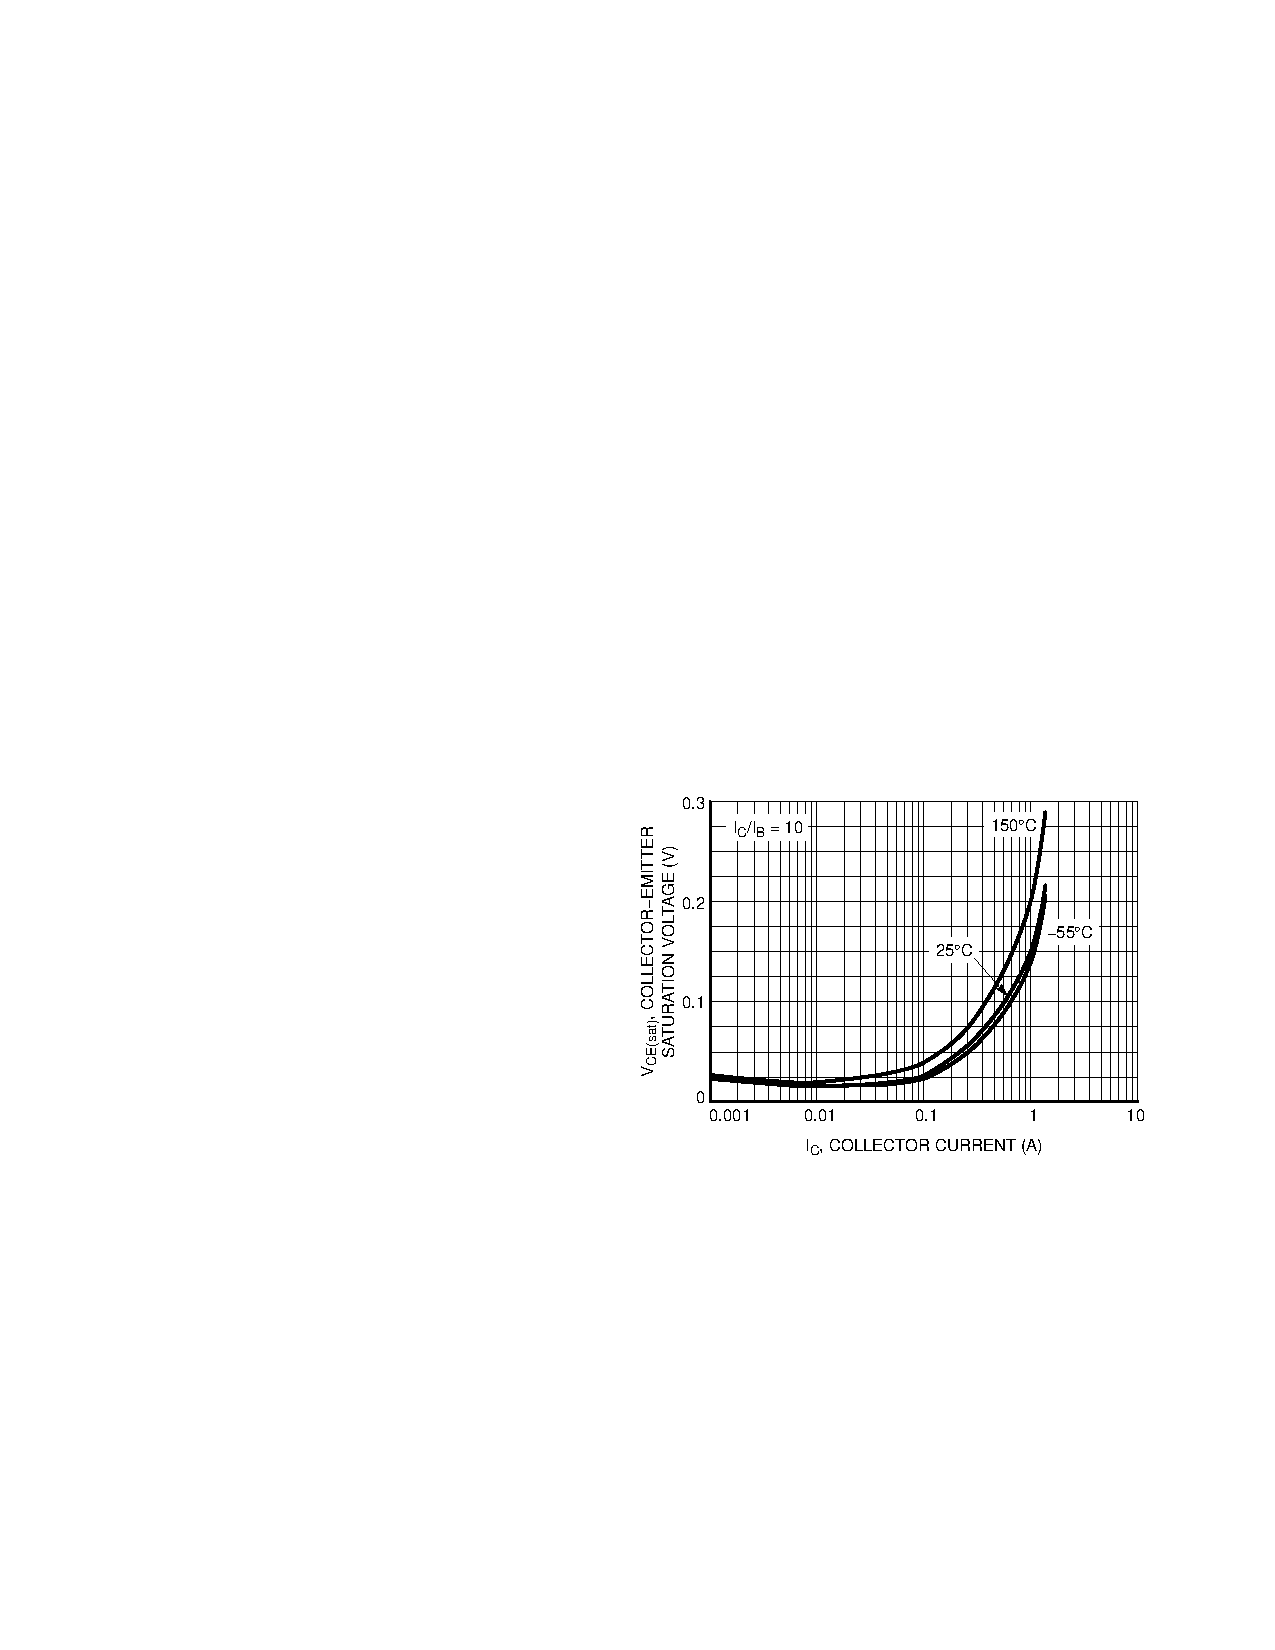
\includegraphics[]{Graphics/Practice 8/BJT/DATASHEET/VCE-IC.pdf}
    \caption{Collector-Emitter Saturation Voltage~\autocite{BD135}}
    \label{fig:VCE_SAT}
\end{figure}


\begin{figure}[H]
    \centering
    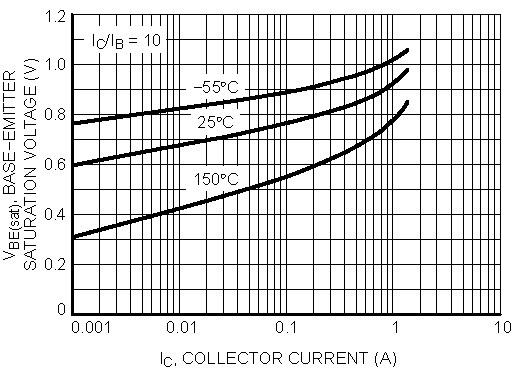
\includegraphics[]{Graphics/Practice 8/BJT/DATASHEET/VBE-IC.pdf}
    \caption{Base-Emitter Saturation Voltage~\autocite{BD135}}
    \label{fig:VBE_SAT}
\end{figure}

\begin{figure}[H]
    \centering
    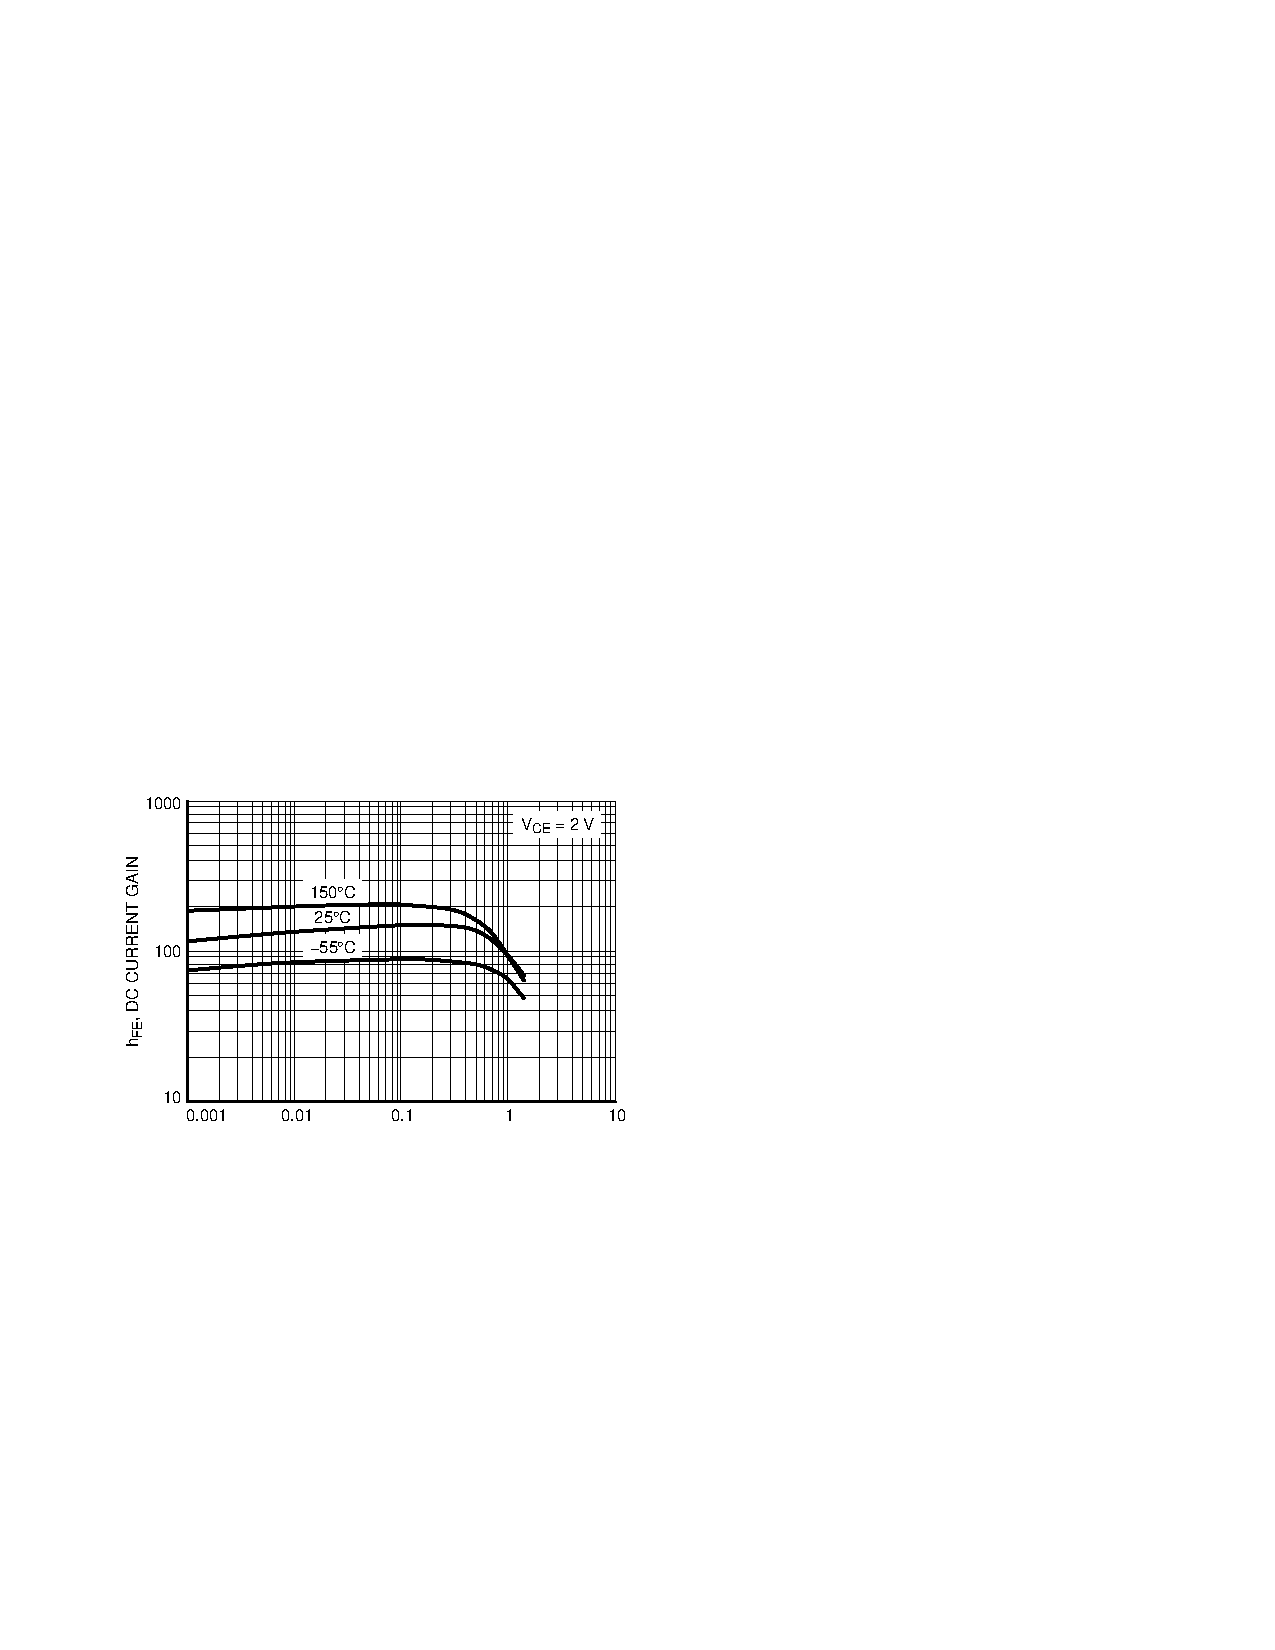
\includegraphics[]{Graphics/Practice 8/BJT/DATASHEET/BETA-IC.pdf}
    \caption{DC Current Gain~\autocite{BD135}}
    \label{fig:DC_GAIN}
\end{figure}

From Figure \ref{fig:VCE_SAT}, we obtain that for a collector current, $I_C \approx 166.67 \; mA$, the $\bm{V_{CE(SAT)} \approx 0.05 \;V}$. Then the \textit{real} value of $I_C$ can be calculated as:

\begin{equation*}
    I_C = \frac{2 \; W}{12 \; V - 0.05} = 167.36 \; mA
\end{equation*}

\noindent From Figure \ref{fig:VBE_SAT} we obtain that, for a $I_C = 167.36 \; mA$ the $\bm{V_{BE(SAT)}} \approx 0.8 \; V$.\medskip

\noindent Finally, from Figure \ref{fig:DC_GAIN} we obtain that, for a $I_C = 167.36 \; mA$, the $\bm{\beta \approx 115}$ \medskip

\noindent With this values, we can calculate the value of $R_B$ following this fashion:

\begin{equation}
    R_B = \frac{V_{OH} - V_{BE(SAT)}}{\dfrac{I_C}{\beta}} = \frac{4.4 - 0.8}{\left( \dfrac{166.67 \; mA}{115} \right)} = 2484 \; \Omega
\end{equation}\medskip

Since the obtained value does not belong to the E-12 series, we will choose $\bm{2.2 \; k\Omega}$, as it will guarantee that enough current is sourced.

\clearpage


























